%% Standalone one/two-page summary for a second/busy reviewer.
%% Self-contained: compiles on its own (pdfLaTeX); the two figures sit next
%% to this file. Numbers match the main report (OVERLEAF_FLAT_BUNDLE/main.tex).
\documentclass[11pt,a4paper]{article}
\usepackage[utf8]{inputenc}
\usepackage[T1]{fontenc}
\usepackage[margin=2.0cm]{geometry}
\usepackage{graphicx}
\usepackage{float}
\usepackage{amsmath, amssymb}
\usepackage{microtype}
\usepackage{caption}
\captionsetup{font=small}
\graphicspath{{./}}
\setlength{\parskip}{0.45em}
\setlength{\parindent}{0pt}
\pagestyle{empty}

\title{\vspace{-1.4cm}When do federated optimisers preserve rare-class signal?\\
\large A regime map for FedAvg, FedProx, and FedNova on imbalanced medical images}
\author{Barbara Koch}
\date{}

\begin{document}
\maketitle
\vspace{-1.2cm}

\textbf{Overview.} This project studies federated learning (FL) under statistical
and system heterogeneity for imbalanced medical image classification. Its
organising finding is a single rule: \emph{rare-class performance is preserved
precisely when the rare client's signal continues to reach the global model.}
Rather than crowning a single best optimiser, the thesis maps \emph{when} each of
FedAvg, FedProx, and FedNova preserves or loses that signal.

\textbf{Problem.} In federated medical settings, rare disease classes are often
concentrated at small or slow (``straggler'') clients. When such a client's update
is delayed, down-weighted, or dropped, its rare-class information can disappear
from the global model. This failure is invisible to accuracy: on DermaMNIST the
majority class (melanocytic nevi) is $66.9\,\%$ of the data, so a model that
ignores the rare classes still scores about $67\,\%$ accuracy. Every comparison
here therefore uses \textbf{macro-F1}, which weights all seven classes equally and
exposes rare-class collapse.

\textbf{Methods (compact).} \emph{Dataset:} DermaMNIST, seven skin-lesion classes,
severely imbalanced (rare classes: dermatofibroma $1.1\,\%$, vascular $1.4\,\%$,
melanoma $11.1\,\%$). \emph{Optimisers:} FedAvg (baseline), FedProx (adds a
proximal term with coefficient $\mu$), FedNova (normalises each client's update by
its local work). \emph{Experimental ladder} of increasing stress: IID baseline
$\rightarrow$ engineered non-IID $\rightarrow$ $\mu$ sensitivity $\rightarrow$
matched two-client rare-client partitions (L1 control vs L4 class-disjoint)
$\rightarrow$ straggler \emph{drop} vs \emph{$\gamma$-inexact} partial-update
acceptance $\rightarrow$ FedNova under learning-rate asymmetry and random work
$\rightarrow$ a weighted-cross-entropy loss-side check.

\textbf{Key results.}
\begin{itemize}\setlength{\itemsep}{0.1em}
\item Under the perfect-storm straggler stress, \emph{accepting} the rare client's
partial update (FedProx${}+{}$$\gamma$-inexact) reaches $0.491$ test macro-F1,
whereas \emph{dropping} it (FedAvg${}+{}$drop) collapses to $0.087$ ---
$\Delta = +0.404$, the largest gap in the study.
\item A controlled four-condition decomposition (Figure~\ref{fig:grid}) shows the
rescue comes almost entirely from $\gamma$-inexact partial-update acceptance
($+0.111$ of a $+0.115$ gain), \emph{not} from the FedProx proximal term
($+0.004$).
\item FedNova is regime-dependent: robust under deterministic learning-rate
asymmetry (up to $+0.131$ macro-F1 at a 50:1 ratio) but brittle under random,
round-to-round work variation (collapsing to $\approx 0.237$).
\item Weighted cross-entropy on FedAvg ($0.505$) matches FedProx with plain
cross-entropy ($0.478$), so FedProx's advantage is \emph{not} simply
class-imbalance correction in disguise --- it acts at the aggregation/protocol
layer, not the loss layer.
\end{itemize}

\begin{figure}[H]
\centering
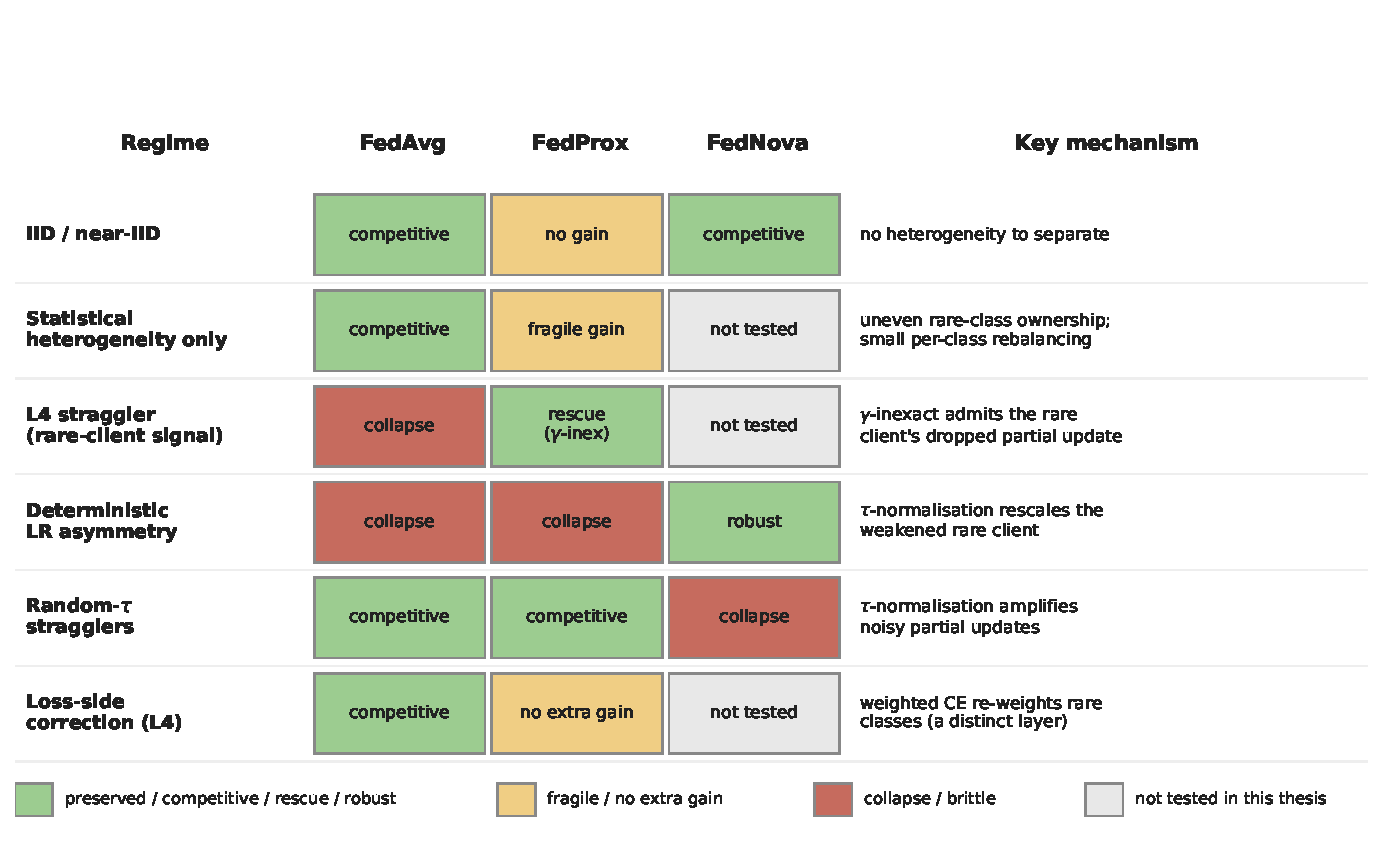
\includegraphics[width=0.95\textwidth]{F_regime_map_summary.pdf}
\caption{Thesis-level synthesis. For each heterogeneity regime, whether each
optimiser preserves rare-class signal (green), gives no extra gain or is fragile
(amber), or collapses (red). The map encodes one rule: rare-class performance is
preserved when rare-client signal reaches the global model.}
\label{fig:regime}
\end{figure}

\textbf{Interpretation.} The practical message is not ``FedProx is always best.''
It is regime-dependent: choose the optimiser \emph{and protocol} that keep
rare-client signal reaching the global model. Under straggler stress, how partial
updates are handled (accept vs drop) can matter more than the proximal term
itself. FedNova helps when client work is stable but asymmetric, yet can fail when
work is random and noisy. The shared failure mode across collapsing settings is
rare lesions being mis-routed into the majority class.

\begin{figure}[H]
\centering
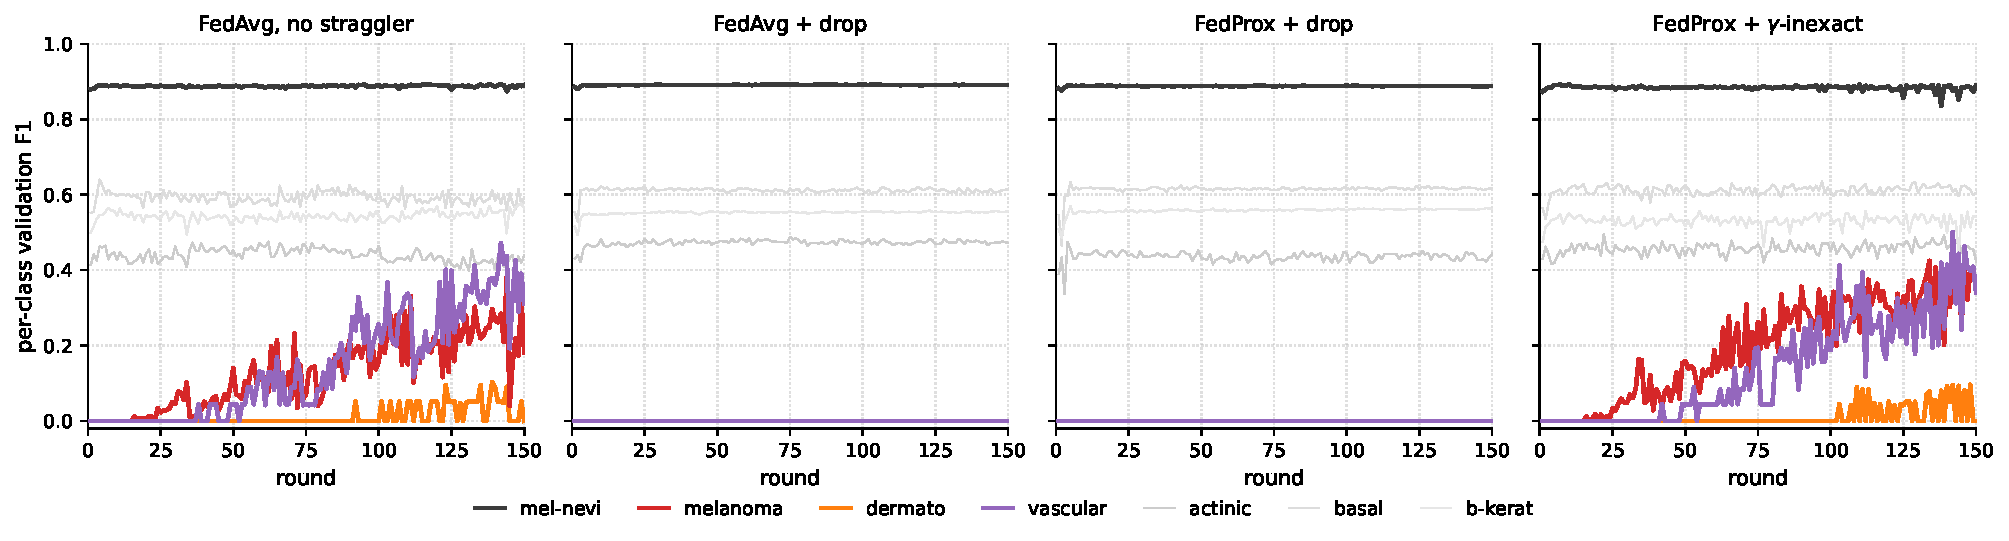
\includegraphics[width=\textwidth]{F_l4_four_condition_per_class_grid.pdf}
\caption{The central result. Per-class validation F1 over training in the
four-condition decomposition. The rare classes (melanoma, dermatofibroma,
vascular) flatline at zero under \emph{both} drop conditions --- FedAvg${}+{}$drop
and FedProx${}+{}$drop alike, so the proximal term alone does not rescue them ---
and recover only under FedProx${}+{}$$\gamma$-inexact, which accepts the rare
client's partial update.}
\label{fig:grid}
\end{figure}

\textbf{Limitations.} Restricted HPC access meant unequal seed counts: headline
comparisons use $n=10$, mechanism probes use $n=3$ (directional, not
significance-tested), and single-seed pilots are labelled as such. The L1/L4,
drop, and straggler settings are deliberate adversarial stress tests, not claims
about naturalistic hospital deployment. DermaMNIST is a low-resolution
($28\times28$) benchmark, so the findings are clinically motivated, not validated.
The FedNova random-work brittleness is an observed failure mode whose precise
cause needs further controlled experiments.

\end{document}
